\documentclass[12pt]{ociamthesis}  % default square logo 
%\documentclass[12pt,beltcrest]{ociamthesis} % use old belt crest logo
%\documentclass[12pt,shieldcrest]{ociamthesis} % use older shield crest logo

%load any additional packages
\usepackage{amssymb}
\usepackage{listings}

\usepackage{color}
 
\definecolor{codegreen}{rgb}{0,0.6,0}
\definecolor{codegray}{rgb}{0.5,0.5,0.5}
\definecolor{codepurple}{rgb}{0.58,0,0.82}
\definecolor{backcolour}{rgb}{0.95,0.95,0.92}
 
\lstdefinestyle{mystyle}{
    backgroundcolor=\color{backcolour},   
    commentstyle=\color{codegreen},
    keywordstyle=\color{magenta},
    numberstyle=\tiny\color{codegray},
    stringstyle=\color{codepurple},
    basicstyle=\footnotesize,
    breakatwhitespace=false,         
    breaklines=true,                 
    captionpos=b,                    
    keepspaces=true,                 
    numbers=left,                    
    numbersep=5pt,                  
    showspaces=false,                
    showstringspaces=false,
    showtabs=false,                  
    tabsize=2,
    language=python
}
 
\lstset{style=mystyle}

%input macros (i.e. write your own macros file called mymacros.tex 
%and uncomment the next line)
%\include{mymacros}

\title{Tugas Chapter \\[1ex]     %your thesis title,
        Pemrograman II}   %note \\[1ex] is a line break in the title

\author{Cecep Gunawan}             %your name
\college{1184092\\[5ex]
Applied Bachelor of Informatics Engineering}  %your college

%\renewcommand{\submittedtext}{change the default text here if needed}
\degree{Politeknik Pos Indonesia}     %the degree
\degreedate{Bandung 2019}         %the degree date

%end the preamble and start the document
\begin{document}

%this baselineskip gives sufficient line spacing for an examiner to easily
%markup the thesis with comments
\baselineskip=18pt plus1pt

%set the number of sectioning levels that get number and appear in the contents
\setcounter{secnumdepth}{3}
\setcounter{tocdepth}{3}


\maketitle                  % create a title page from the preamble info
\include{section/dedication}        % include a dedication.tex file
\begin{acknowledgements}
Pertama-tama kami panjatkan puji dan syukur kepada Allah SWT yang telah memberikan rahmat dan hidayah-Nya sehingga Modul Praktikum ini dapat diselesaikan.
\end{acknowledgements}   % include an acknowledgements.tex file
\begin{abstract}
	Modul Praktikum ini dibuat dengan tujuan memberikan acuan, bagi mahasiswa dan dosen
	Pengajar Mata Kuliah. Pada intinya buku ini menjelaskan secara lengkap tentang Standar penilian mata kuliah pemrograman II
	di Program Studi D4 Teknik Informatika, dan juga mengatur mekanisme, teknik penulisan, serta
	penilaiannya.Dengan demikian diharapkan semua pihak yang terlibat dalam aktivitas belajar dan mengajar
	berjalan lancar dan sesuai dengan standar.
\end{abstract}          % include the abstract

\begin{romanpages}          % start roman page numbering
\tableofcontents            % generate and include a table of contents
\listoffigures              % generate and include a list of figures
\end{romanpages}            % end roman page numbering

%now include the files of latex for each of the chapters etc
\chapter{Teori, Sejarah, \& Instalasi Python}
\section{Teori}
Python adalah bahasa pemrograman interpretatif multiguna, python lebih menekankan pada keterbacaan kode agar lebih mudah untuk memahami sintaks.
\section{Sejarah Python}
Python diciptakan oleh Guido van Rossum pertama kali di centrum wiskunde \& informatica (CWI) di Belanda pada awal tahun 1990-an. bahasa yang terinpirasi dari bahasa pemograman ABC, hingga sampai saat ini Guido van Rossum menjadi penulis utama untuk phyton.
Tahun 1995 masih melanjutkan pembuatan phyton di Corporation for National Research Initiative (CNRI) di Virginia Amerika yang meriliskan beberapa bahasa phyton. Diantaranya :
\begin{enumerate}
	\item Python 1.0
	\\ Diliris pada januari tahun 1994
	\item Python 2.0
	\\ Diliris pada 16 Oktober tahun 2000
	\item Python 3.0 
	\\ Diliris pada 3 Desember tahun 2008
\end{enumerate}  
\subsubsection{Penggunaan Python di Perusahaan}
Salah satu bahasa yang banyak dipakai dalam sebuah perusahaan hingga saat ini yaitu bahasa pemograman python,  contoh penggunaan dalam perusahaan yaitu : 
\begin{enumerate}
\item Facebook
\\ Menggunakan framework python "Tornado" yang digunakan untuk menampilkan timeline
\item Instagram 
\\ Menggunakan framework python "Django" yang digunakan sebagai mesin pengelola sisi server dari aplikasi
\item Rasberry pi 
\\ Merupakan perangkat komputer mini yang digunakan sebagi mikrokontroler, bahasa yang digunakannya adalah python
\item NASA
\\ Badan antariksa Amerika ini menggunakan Python untuk bidang sainsnya.
\end{enumerate}
\subsubsection{Perbedaan Python 2 dan 3}
	Python 2 dipublikasikan pada akhir tahun 2000, dinilai lebih transparan dan inklusif untuk pengembangan software ketimbang versi sebelumnya. didukung dengan adanya PEP – Python Enhancement Proposal, dan dilengkapi dengan berbagai fitur programatikal seperti cycle-detecting garbage collector untuk mengotomasi manajemen memori. 
\\ Python 3 merupakan versi yang saat  ini dibuat masih aktif, versi ini banyak perubahan yang dirilis akhir tahun 2008. Fokus dari Python 3 itu sendiri adalah untuk melakukan perapian pada codebase dan menghapuskan duplikasi (redundancy). Python 3 mengalami hambatan pada pengadopsiannya, yang mengakibatkan tidak adanya backwards compatibility dengan Python 2.
\\	 
perbedaan yang mencolok terletak pada : 
\begin{enumerate}
\item Syntak
\item Pembagian pada integer
\end{enumerate}

\section{Instalasi}
\subsection{Instalasi Anaconda}
Berikut ini merupakan tutorial cara menginstalasi Anaconda, yang telah di download di www.anaconda.com setelah itu ikuti langkah-langkah dibawah ini.

	\begin{figure}
	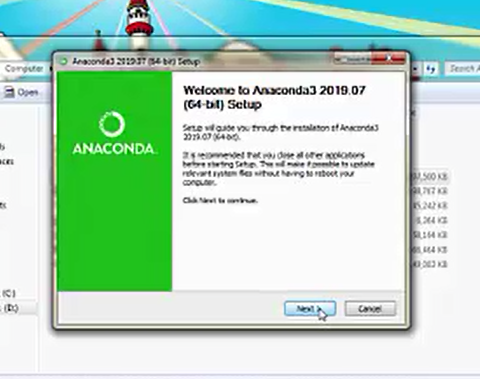
\includegraphics[scale=0.5]{section/1.png}
	\centering
	\caption{Tahap Instalasi 1}
	\end{figure}
	
	\begin{figure}
	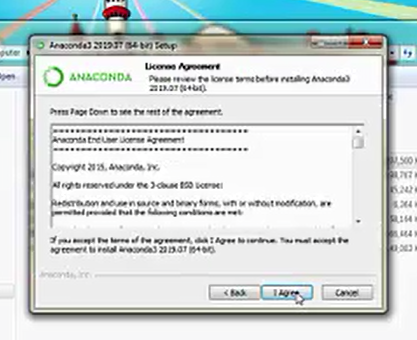
\includegraphics[scale=0.5]{section/2.png}
	\centering
	\caption{Tahapan Instalasi 2}
	\end{figure}

	\begin{figure}
	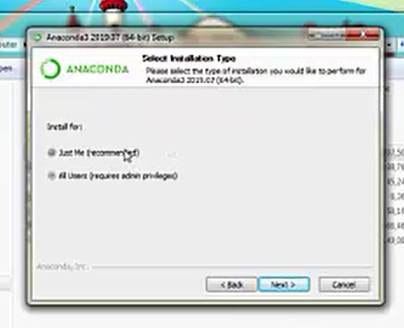
\includegraphics[scale=0.5]{section/3.png}
	\centering
	\caption{Tahapan Instalasi 3}
	\end{figure}

	\begin{figure}
	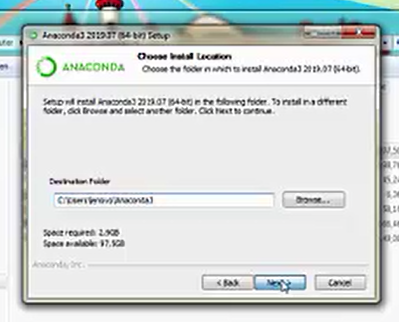
\includegraphics[scale=0.5]{section/4.png}
	\centering
	\caption{Tahapan Instalasi 4}
	\end{figure}

	\begin{figure}
	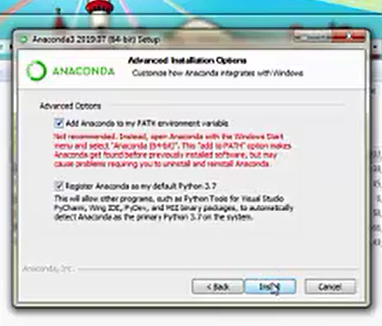
\includegraphics[scale=0.5]{section/5.png}
	\centering
	\caption{Tahapan Instalasi 5}
	\end{figure}

	\begin{figure}
	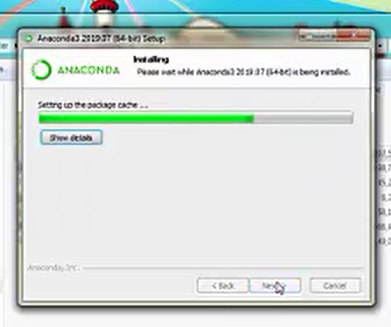
\includegraphics[scale=0.5]{section/6.png}
	\centering
	\caption{Tahapan Instalasi 6}
	\end{figure}

	\begin{figure}
	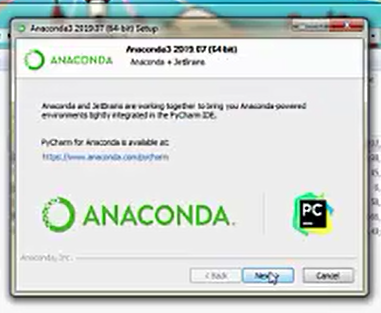
\includegraphics[scale=0.5]{section/7.png}
	\centering
	\caption{Tahapan Instalasi 7}
	\end{figure}

	\begin{figure}
	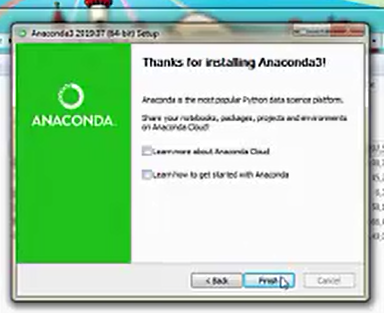
\includegraphics[scale=0.5]{section/8.png}
	\centering
	\caption{Tahapan Instalasi 8}
	\end{figure}

	\begin{figure}
	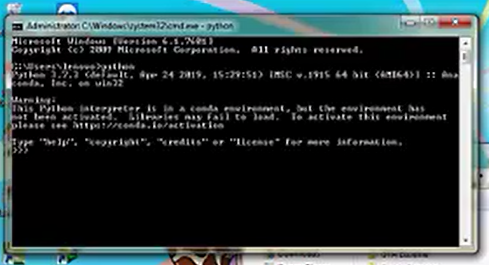
\includegraphics[scale=0.5]{section/9.png}
	\centering
	\caption{Tahapan Instalasi 9}
	\end{figure}

\subsection{Intalasi PIP}
Langkah-langkah mengisntall PIP

	\begin{figure}
	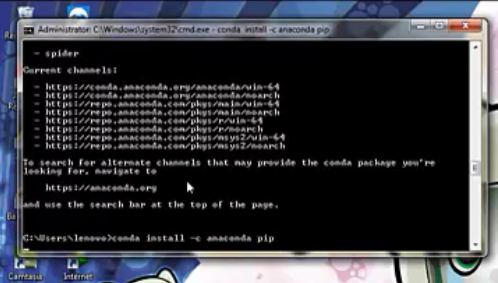
\includegraphics[scale=0.5]{section/pip1}
	\centering
	\caption{Ketik printah : conda install -c anaconda pip}
	\end{figure}
	
	\begin{figure}
	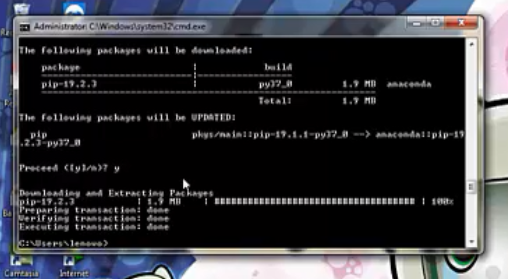
\includegraphics[scale=0.5]{section/pip2}
	\centering
	\caption{Tunggu hingga selesai}
	\end{figure}
	
\section{Setting Environment}
Langkah-langkah seperti ini : 

	\begin{figure}
	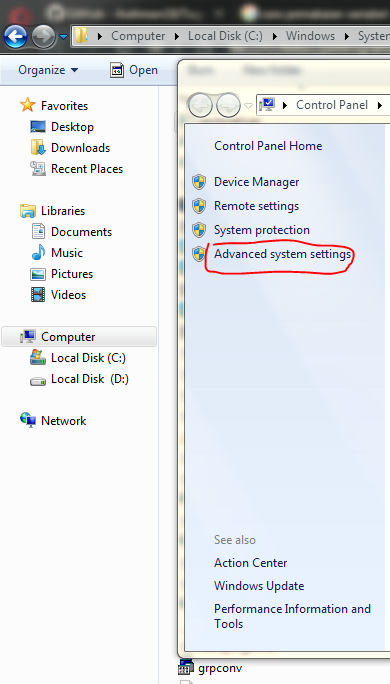
\includegraphics[scale=0.5]{section/envirotment1}
	\centering
	\caption{pilih advanced system setting}
	\end{figure}	
	
	\begin{figure}
	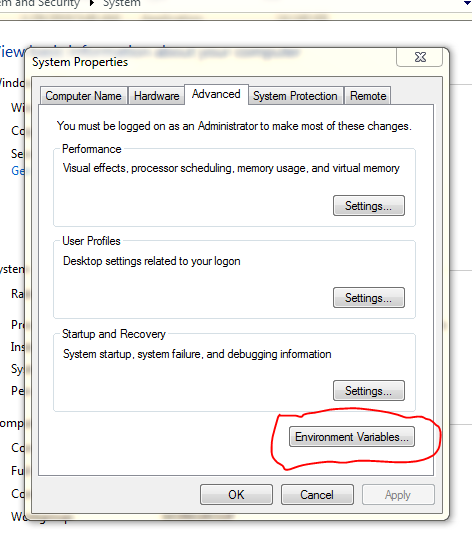
\includegraphics[scale=0.5]{section/envirotment2}
	\centering
	\caption{pilih envirotmet variabel}
	\end{figure}
	
	\begin{figure}
	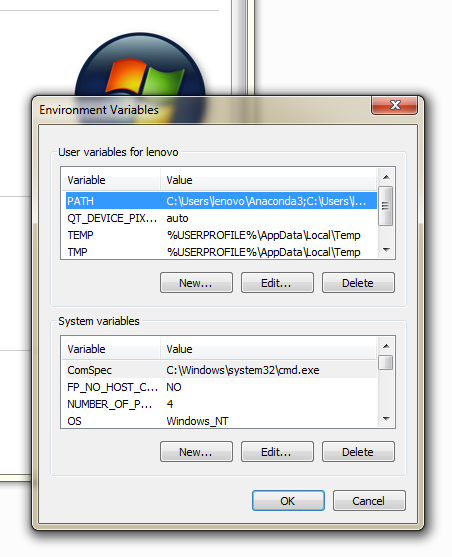
\includegraphics[scale=0.5]{section/envirotment3}
	\centering
	\caption{setting environment}
	\end{figure}
\section{Entrepreter atau CLI melalui terminal atau cmd windows}
pada tahap ini, dibutuhkanya cmd sebagai bahan pembelajaran dari mulai cek status python yang sudah terbaru, hingga proses pengupdatetan seperti contoh dibawah ini:

	\begin{figure}
	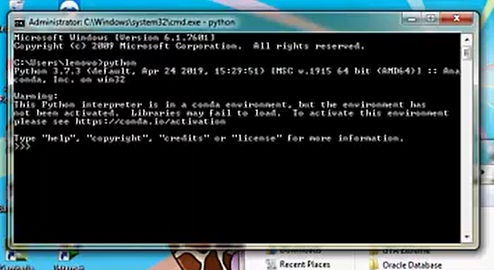
\includegraphics[scale=0.5]{section/13.png}
	\centering
	\caption{Tahapan Cek python}
	\end{figure}

	\begin{figure}
	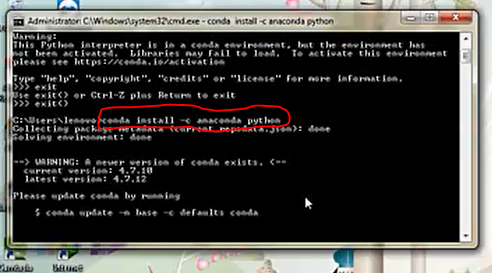
\includegraphics[scale=0.5]{section/14.png}
	\centering
	\caption{Tahapan pengudatetan}
	\end{figure}

\section{Mengupdate Spyder}
Pada langkah ini, dibutuhkan sebuah command Prompt dengan megetikkan
\\ conda install -c anaconda spyder

	\begin{figure}
	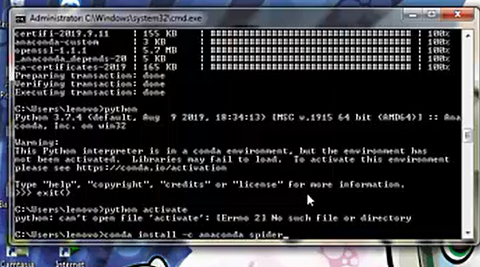
\includegraphics[scale=0.5]{section/10.png}
	\centering
	\caption{Tahapan update spyder}
	\end{figure}

\section{Menjalankan Hello World}
Pada langkah ini harus di siapkan spyder yang digunakan sebagai text editor yang membantu menerjemahkan bahasa pemograman python, diantaranya sebagai berikut :

	\begin{figure}
	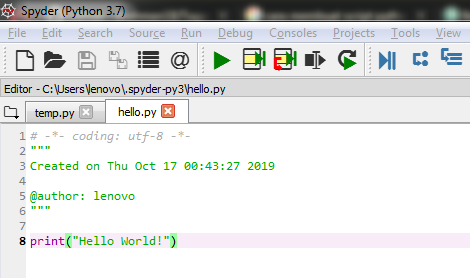
\includegraphics[scale=0.5]{section/11.png}
	\centering
	\caption{Syntak hello world}
	\end{figure}

	\begin{figure}
	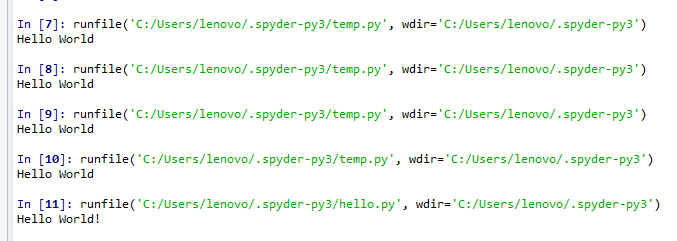
\includegraphics[scale=0.5]{section/12.png}
	\centering
	\caption{menampilkan hello world}
	\end{figure}


\section{Menjalankan Script Otomatis Login Aplikasi Akademik}
Pada langkah pertama instal selenium terlebih dahulu seperti contoh ini :

	\begin{figure}
	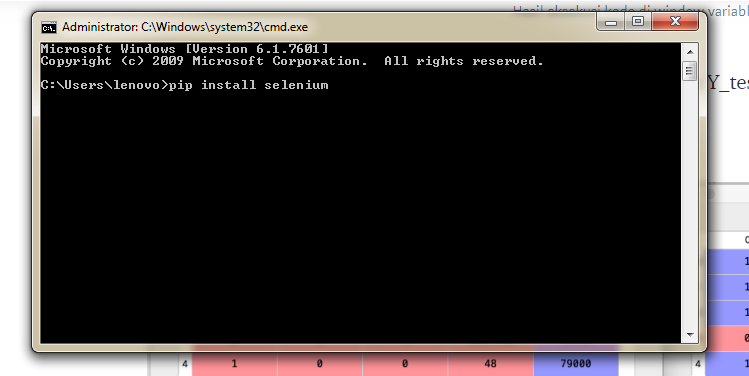
\includegraphics[scale=0.5]{section/selenium.png}
	\centering
	\caption{Install selenium}
	\end{figure}

	\begin{figure}
	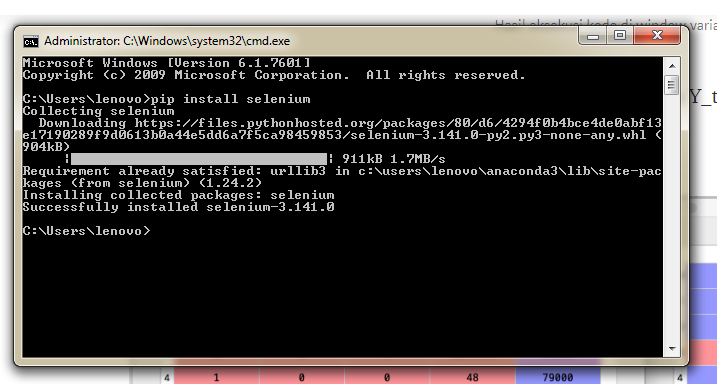
\includegraphics[scale=0.5]{section/proses_selenium}
	\centering
	\caption{Tahap instalasi selenium}
	\end{figure}
	
	\begin{figure}
	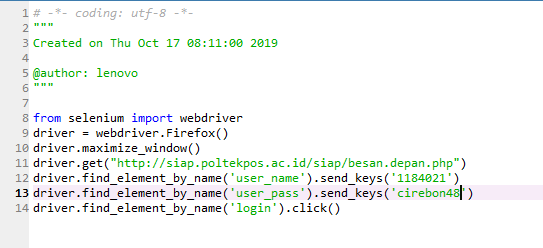
\includegraphics[scale=0.5]{section/login_otomatis}
	\centering
	\caption{Syntak pada spyder untuk otomatis login}
	\end{figure}
	
	\begin{figure}
	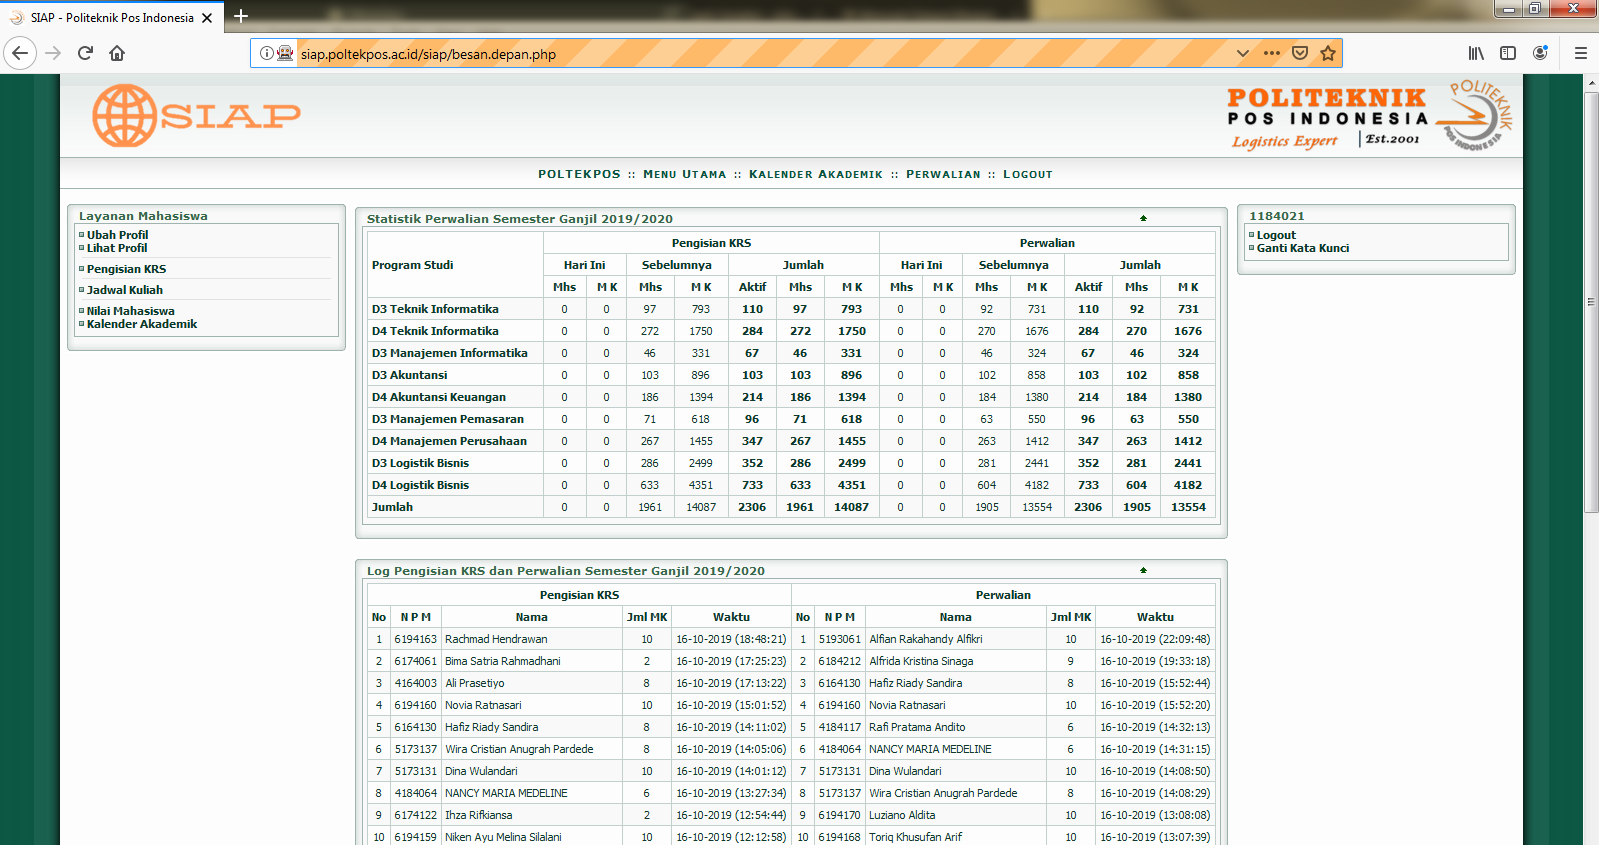
\includegraphics[scale=0.3]{section/hasil.png}
	\centering
	\caption{hasil}
	\end{figure}

\section{Variable Explorer}
Variabel explorer digunakan sebagai bawaan untuk mengedit daftar, string, kamus, array NumPy, Pandas DataFrames, dan banyak lagi, dan dapat juga histogram, plot, atau bahkan menampilkan beberapa di antaranya sebagai gambar RGB. Bisa dicek dengan mengklik variabel explorer pada spyder.

	\begin{figure}
	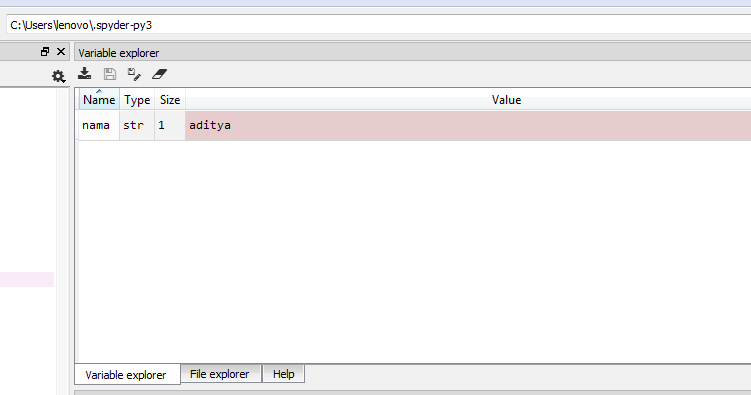
\includegraphics[scale=0.3]{section/variabel_explorer.png}
	\centering
	\caption{cek variabel explorer}
	\end{figure}
	
\section{Identasi}
Indentasi adalah bagian paragraf yang menjorok ke dalam pada baris-baris
paragraf, penulisan kode python tidak memakai curly brackets ”{}” sehingga
cara membedakan blok program digunakan identasi.
jenis error identasi yaitu IndentationError: expected an indented block.
artinya ini berarti fungsi if memerlukan indentasi untuk membedakan blok
kode.

	\begin{figure}
	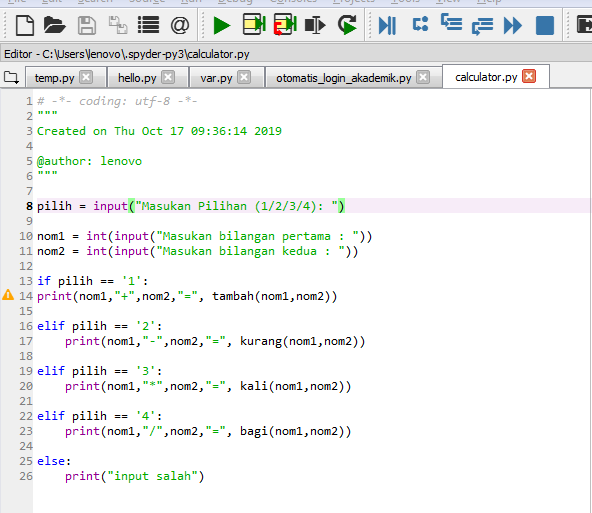
\includegraphics[scale=0.5]{section/salah.png}
	\centering
	\caption{syntak eror identasi}
	\end{figure}
	
	\begin{figure}
	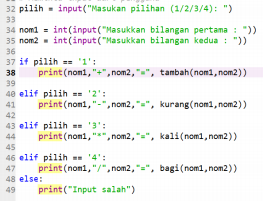
\includegraphics[scale=1.5]{section/benar.png}
	\centering
	\caption{cek variabel explorer}
	\end{figure}
\chapter{Pemrograman Dasar}
\section{Teori}
\begin{enumerate}
\item
Variabel merupakan tempat menyimpan data, sedangkan tipe data adalah jenis data yang tersimpan dalam variabel, Variabel bersifat mutable, artinya nilainya bisa berubah-ubah. Variabel memiliki beberapa jenis termasuk : 
	\begin{enumerate}
	\item
	Variabel global, yaitu variabel yang bisa diakses dengan semua fungsi
	\item
	Variabel local, yaitu variabel yang bisa diakses dalam fungsi dan tempat variabel berada.
	\item
	Variabel build-in, yaitu variabel yang sudah termasuk ada dalam python
	\end{enumerate}
\item
Dengan menuliskan sricpt seperti ini : \\
A=input("Cecep") \\
maka untuk menampilkan ketikan perintah dibawah ini : \\
print("halo", Cecep "Apa Kabar")
\item
Operator dasar matematika adalah : \\
	1. + (pertambahan)\\
	2. - (pengurangan)\\
	3. / (pembagian)\\
	4. x (perkalian)\\
\begin{enumerate}
\item
Untuk merubahnya menjadi integer gunakanlah kode int() \\ 
Sebagai contoh : \\
b=876 \\ integer = int(b) <sricpt konversi dari string ke integer> \\
print(integer) <untuk mencetak hasilnya> \\
\item
Untuk merubahnya menjadi string gunakanlah kode str() \\
sebagai contoh : \\
r=747 \\ string = str(r) <sricpt konversi dari integer ke string> \\
print(string) <untuk mencetak hasilnya> \\ 
\end{enumerate}
\item
Ada 2 perulangan yaitu while loop dan for loop. 
\begin{enumerate}
\item
While loop adalah perulangan yang selalu dieksekusi selama kondisi bernilai benar(true).
\item
For loop adalah perulangan yang memiliki kemampuan untuk mengulangi item dari urutan apapun seperti list atau string
\end{enumerate} 
1. Contoh sricpt pada while loop : \\
Count = 0 \\
while (count < 9): \\
print'the count is:',count \\
Count = count+1 \\
print("Good Bye!") \\ \\
2. Contoh penerapan for loop : \\
Nomer=[1,2,3,4,5] \\
For x in nomer: \\
Print(x)\\
\item
Ada 3 macam kondisi diantaranya : 
\begin{enumerate}
\item
If \\ adalah suatu kondisi yang bernilai benar atau salah, jika dalam statmennt bernilai benar akan dijalankan, tetapi sebaliknya jika statmennt bernilai salah maka tidak akan dijalankan (eror). 
\item
If - Else \\ adalah suatu kondisi bernilai benar maka statment didalam if akan dieksekusi dan jika bernilai false maka statment yang dieksekusi adalah statment didalam else
\item
If - Elif - Else \\ adalah suatu kondisi Elif, lanjutan dari percabangan  if dengan kondisi ini menyebabkan beberapa kemungkinan statment yang terjadi.
\end{enumerate}
1. Sebagai contoh script IF yang bernilai true. \\
x=1 \\
IF x >0; \\
Print("Nilai \%x adalah besar dari 0"\%x) \#Nilai 1 adalah besar dari 0 \\
Kondisi diatas bernilai true, karena nilai x(1) lebih besar dari 0. \\ \\
Sedangkan script di bawah ini merupakan contoh dari suatu kondisi bernilai false. \\
x=1 \\
IF x >2; \\
Print("Nilai \%x adalah besar dari 0"\%x) \\
Kondisi diatas bernilai false, maka outputan tidak akan muncul.\\ \\
2. Sebagai contoh script IF-Else : \\
x=1 \\
IF x >5: \\
Print("Nilai \%d adalah besar dari 5"\%x) \\
Else:
Print("Nilai \%d adalah kecil dari \%"\%x) \\ 
\# Nilai 1 adalah kecil dari 5 \\ sebaliknya, ubahlah nilai x menjadi 20.\\
x=20 \\
IF x >5:\\
Print("Nilai \%d adalah besar dari 5"\%x)\\
Else: \\
Print("Nilai \%d adalah kecil dari 5"\%x)\\\\
3. Sebagai contoh script IF ELIF ELSE : \\
x=5\\
if x <5:\\
Print("Nilai \%d adalah kecil dari 5"\%x)\\
elif x==5:\\
Print("Nilai \%d adalah sama dengan 5"\%x)\\
else: \\
Print("Nilai \%d adalah besar dari 5"\%x)\\
\item
diantara sintak-sintak eror yang ditemui antara lain :
\begin{enumerate}
\item
TypeError:unsupported operand type(s) for +:'int' and 'str' \\ penangann error ini bisa ditandai menggunakan casting operand kedua menjadi integer
\item
TypeError:can only concatenate str(not"int") to str \\ penanganan ini ditandai dengan menggunakan casting operand kedua menjadi string. 
\end{enumerate}
\item
Try Except adalah bentuk penanganan error yang terdapat dalam bahasa pemograman (python). Contoh penanganannya : \\
Setiap bilangan yang dibagi 0 akan terjadi error karena ini merupakan ketentuan dari awal dan tidak bisa dieskekusi, tetapi dengan menggunakan try except dapat ditangani walaupun akan terjadi error dibawah ini : \\
x=0\\
Try:\\
x=9/0\\
Except exception,e;\\
print e\\
print x=1 \\
Maka akan muncul peringatan error integer devision or modulo by zero 1
\end{enumerate}

\section{Ketrampilan Pemrograman}
Buat program di python dengan ketentuan:
\begin{enumerate}
\item
Berikut ini merupakan soal praktikum no 1 dengan soal sebagai berikut : \\
Buatlah luaran huruf yang dirangkai dari tanda bintang, pagar atau plus dari NPM kita.
Tanda bintang untuk NPM mod 3=0, tanda pagar untuk NPM mod 3 =1, tanda plus untuk NPM mod3=2.
Contoh sricpt : 
\begin{verbatim}
# -*- coding: utf-8 -*-
"""
Created on Tue Oct 22 21:29:47 2019

@author: lenovo
"""

print("***   ***   *******   ******  ******  ******  ******  ");
print("***   ***   **   **  **   **  **  **  **  **      **  ");
print("***   ***    ****   ********  **  **  ******  ******  ");
print("***   ***   **   **       **  **  **      **  **      ");
print("***   ***   *******       **  ******  ******  ******  ");
\end{verbatim}
\item
Berikut ini hasil script dari soal no 2 praktikum
\begin{verbatim}
# -*- coding: utf-8 -*-
"""
Created on Tue Oct 22 21:04:07 2019

@author: lenovo
"""

npm=int(input("masukan npm anda : "))
TwoLastDigit=abs(npm)%100 # modulus menetukan ambil 2 digit terakhir
for i in range(TwoLastDigit):
    print("Halo, ", npm, " Apa kabar ?")
\end{verbatim}
Maka hasil Outputnya adalah menampilkan 'Halo, 1184021 Apa kabar ?' sebanyak 21x tampilan. 
\begin{verbatim}
masukan npm anda : 1184092
Halo,  1184092  Apa kabar ?
Halo,  1184092  Apa kabar ?
Halo,  1184092  Apa kabar ?
Halo,  1184092  Apa kabar ?
Halo,  1184092  Apa kabar ?
Halo,  1184092  Apa kabar ?
Halo,  1184092  Apa kabar ?
Halo,  1184092  Apa kabar ?
Halo,  1184092  Apa kabar ?
Halo,  1184092  Apa kabar ?
Halo,  1184092  Apa kabar ?
Halo,  1184092  Apa kabar ?
Halo,  1184092  Apa kabar ?
Halo,  1184092  Apa kabar ?
Halo,  1184092  Apa kabar ?
Halo,  1184092  Apa kabar ?
Halo,  1184092  Apa kabar ?
Halo,  1184092  Apa kabar ?
Halo,  1184092  Apa kabar ?
Halo,  1184092  Apa kabar ?
Halo,  1184092  Apa kabar ?
Halo,  1184092  Apa kabar ?
Halo,  1184092  Apa kabar ?
Halo,  1184092  Apa kabar ?
Halo,  1184092  Apa kabar ?
Halo,  1184092  Apa kabar ?
Halo,  1184092  Apa kabar ?
Halo,  1184092  Apa kabar ?
Halo,  1184092  Apa kabar ?
Halo,  1184092  Apa kabar ?
Halo,  1184092  Apa kabar ?
Halo,  1184092  Apa kabar ?
Halo,  1184092  Apa kabar ?
Halo,  1184092  Apa kabar ?
Halo,  1184092  Apa kabar ?
Halo,  1184092  Apa kabar ?
Halo,  1184092  Apa kabar ?
Halo,  1184092  Apa kabar ?
Halo,  1184092  Apa kabar ?
Halo,  1184092  Apa kabar ?
Halo,  1184092  Apa kabar ?
Halo,  1184092  Apa kabar ?
Halo,  1184092  Apa kabar ?
Halo,  1184092  Apa kabar ?
Halo,  1184092  Apa kabar ?
Halo,  1184092  Apa kabar ?
Halo,  1184092  Apa kabar ?
Halo,  1184092  Apa kabar ?
Halo,  1184092  Apa kabar ?
Halo,  1184092  Apa kabar ?
Halo,  1184092  Apa kabar ?
Halo,  1184092  Apa kabar ?
Halo,  1184092  Apa kabar ?
Halo,  1184092  Apa kabar ?
Halo,  1184092  Apa kabar ?
Halo,  1184092  Apa kabar ?
Halo,  1184092  Apa kabar ?
Halo,  1184092  Apa kabar ?
Halo,  1184092  Apa kabar ?
Halo,  1184092  Apa kabar ?
Halo,  1184092  Apa kabar ?
Halo,  1184092  Apa kabar ?
Halo,  1184092  Apa kabar ?
Halo,  1184092  Apa kabar ?
Halo,  1184092  Apa kabar ?
Halo,  1184092  Apa kabar ?
Halo,  1184092  Apa kabar ?
Halo,  1184092  Apa kabar ?
Halo,  1184092  Apa kabar ?
Halo,  1184092  Apa kabar ?
Halo,  1184092  Apa kabar ?
Halo,  1184092  Apa kabar ?
Halo,  1184092  Apa kabar ?
Halo,  1184092  Apa kabar ?
Halo,  1184092  Apa kabar ?
Halo,  1184092  Apa kabar ?
Halo,  1184092  Apa kabar ?
Halo,  1184092  Apa kabar ?
Halo,  1184092  Apa kabar ?
Halo,  1184092  Apa kabar ?
Halo,  1184092  Apa kabar ?
Halo,  1184092  Apa kabar ?
Halo,  1184092  Apa kabar ?
Halo,  1184092  Apa kabar ?
Halo,  1184092  Apa kabar ?
Halo,  1184092  Apa kabar ?
Halo,  1184092  Apa kabar ?
Halo,  1184092  Apa kabar ?
Halo,  1184092  Apa kabar ?
Halo,  1184092  Apa kabar ?
Halo,  1184092  Apa kabar ?
Halo,  1184092  Apa kabar ?
\end{verbatim}
\item
Buatlah program hello word dengan input nama yang disimpan dalam sebuah variabel string bernama \textbf{NPM} dan beri luaran output berupa tiga karakter belakang dari NPM sebanyak penjumlahan tiga dijit tersebut. berikut ini merupakan script dari soal ini.
\begin{verbatim}
# -*- coding: utf-8 -*-
"""
Created on Tue Oct 22 22:19:12 2019
@author: lenovo
"""
npm=int(input("Masukan NPM : "))
key=str(npm%1000)
print("Hallo, "+str(npm)[4]+str(npm)[5]+str(npm)[6]+" Apa kabar?")
for i in range(int(str(npm)[4])+int(str(npm)[5])+int(str(npm)[6])-1):
         print("Hallo, "+str(npm)[4]+str(npm)[5]+str(npm)[6]+" Apa kabar?")
\end{verbatim}
Maka hasilnya adalah 3x muncul "Hallo, 092 Apa Kabar?" 
\begin{verbatim}
Masukan NPM : 1184092
Hallo, 092 Apa kabar?
Hallo, 092 Apa kabar?
Hallo, 092 Apa kabar?
Hallo, 092 Apa kabar?
Hallo, 092 Apa kabar?
Hallo, 092 Apa kabar?
Hallo, 092 Apa kabar?
Hallo, 092 Apa kabar?
Hallo, 092 Apa kabar?
Hallo, 092 Apa kabar?
Hallo, 092 Apa kabar?
\end{verbatim}
\item
Buatlah program hello word dengan input nama yang disimpan dalam sebuah variabel string bernama \textbf{NPM} dan beri luaran output berupa digit ketiga dari belakang dari variabel NPM. Berikut sricpt nya :
\begin{verbatim}
# -*- coding: utf-8 -*-
"""
Created on Tue Oct 22 22:43:26 2019
@author: lenovo
"""
npm=int(input("Masukan NPM : "))
key=npm%1000
str_key=str(key)
print("hello, "+str_key[0]+" Apa kabar ?")
\end{verbatim}
Maka Hasil nya adalah sebagai berikut :
\begin{verbatim}
Masukan NPM : 1184092
hello, 2 Apa kabar ?
\end{verbatim}
\item
Pada soal no 5 ini merupakan penggunanan perulangan dan kodisi. contoh penerapan dalam sricpt nya adalah sebagai berikut :
\begin{verbatim}
# -*- coding: utf-8 -*-
"""
Created on Tue Oct 22 22:47:07 2019
@author: lenovo
"""
i=0
npm=input("Masukan NPM : ")
while i<1:
    if len(npm) < 7:
        print("NPM Kurang dari 7 digit")
        npm=input("Masukan NPM : ")
    elif len(npm) > 7:
        print("NPM lebih dari 7 digit")
        npm=input("Masukan NPM : ")
    else:
        i=1
a=npm[0]
b=npm[1]
c=npm[2]
d=npm[3]
e=npm[4]
f=npm[5]
g=npm[6]
for x in a,b,c,d,e,f,g:
    print(x,end = ""),
\end{verbatim}
Maka akan keluar outputan : \\
Masukan NPM : 1184092 \\
1184092
\item
Setelah dilakukan perulangan maka seluruh variabel dijumlahkan . maka sricpt nya sebagai berikut :
\begin{verbatim}
# -*- coding: utf-8 -*-
"""
Created on Tue Oct 22 20:58:14 2019
@author: lenovo
"""
i=0
npm=input("Masukan NPM : ")
while i<1:
    if len(npm) < 7:
        print("NPM Kurang dari 7 digit")
        npm=input("Masukan NPM : ")
    elif len(npm) > 7:
        print("NPM lebih dari 7 digit")
        npm=input("Masukan NPM : ")
    else:
        i=1
a=npm[0]
b=npm[1]
c=npm[2]
d=npm[3]
e=npm[4]
f=npm[5]
g=npm[6]
y=0
for x in a,b,c,d,e,f,g:
    y+=int(x)
    print(y)
\end{verbatim}
Hasilnya adalah seperti ini :
\begin{verbatim}
Masukan NPM : 1184092
1
2
10
14
14
16
17
\end{verbatim}
\item 
Sama hal-nya pada no 6, yang membedakannya pada no 7 ini adalah veriabel tersebut dikalikan dengan aritmatikan perkalian, contohnya sricpt sebagai berikut : 
\begin{verbatim}
# -*- coding: utf-8 -*-
"""
Created on Tue Oct 22 23:02:17 2019
@author: lenovo
"""
i=0
npm=input("Masukan NPM : ")
while i<1:
    if len(npm) < 7:
        print("NPM Kurang dari 7 digit")
        npm=input("Masukan NPM : ")
    elif len(npm) > 7:
        print("NPM lebih dari 7 digit")
        npm=input("Masukan NPM : ")
    else:
        i=1
a=npm[0]
b=npm[1]
c=npm[2]
d=npm[3]
e=npm[4]
f=npm[5]
g=npm[6]
conv=1
for x in a,b,c,d,e,f,g:
    conv*=int(x)
    print(conv)
\end{verbatim}
Maka Hasilnya adalah
\begin{verbatim}
Masukan NPM : 1184092
1
1
8
32
0
0
0
\end{verbatim}
\item
Dilakukannya Proses yang outputannya vertikal, script nya berupa seperti ini :
\begin{verbatim}
# -*- coding: utf-8 -*-
"""
Created on Tue Oct 22 21:13:37 2019
@author: lenovo
"""
i=0
npm=input("Masukan NPM : ")
while i<1:
    if len(npm) < 7:
        print("NPM Kurang dari 7 digit")
        npm=input("Masukan NPM : ")
    elif len(npm) > 7:
        print("NPM lebih dari 7 digit")
        npm=input("Masukan NPM : ")
    else:
        i=1
a=npm[0]
b=npm[1]
c=npm[2]
d=npm[3]
e=npm[4]
f=npm[5]
g=npm[6]
for x in a,b,c,d,e,f,g:
    print(x)
\end{verbatim}
Maka Hasilnya adalah : 
\begin{verbatim}
Masukan NPM : 1184092
1
1
8
4
0
9
2
\end{verbatim}
\item
Menampilkan digit genap script nya adalah : 
\begin{verbatim}
# -*- coding: utf-8 -*-
"""
Created on Tue Oct 22 23:10:26 2019
@author: lenovo
"""
i=0
npm=input("Masukan NPM : ")
while i<1:
    if len(npm) < 7:
        print("NPM Kurang dari 7 digit")
        npm=input("Masukan NPM : ")
    elif len(npm) > 7:
        print("NPM lebih dari 7 digit")
        npm=input("Masukan NPM : ")
    else:
        i=1
a=npm[0]
b=npm[1]
c=npm[2]
d=npm[3]
e=npm[4]
f=npm[5]
g=npm[6]
conv=1
for x in a,b,c,d,e,f,g:
    if int(x)%2==0:
        if int(x)==0:
            x=""
    print(x,end = "")
\end{verbatim}
Maka Hasilnya adalah :
\begin{verbatim}
Masukan NPM : 1184092
8402
\end{verbatim}
\item
Dan hasil dari proses ganjil , script berupa :
\begin{verbatim}
# -*- coding: utf-8 -*-
"""
Created on Tue Oct 22 23:16:50 2019
@author: lenovo
"""
i=0
npm=input("Masukan NPM : ")
while i<1:
    if len(npm) < 7:
        print("NPM Kurang dari 7 digit")
        npm=input("Masukan NPM : ")
    elif len(npm) > 7:
        print("NPM lebih dari 7 digit")
        npm=input("Masukan NPM : ")
    else:
        i=1
a=npm[0]
b=npm[1]
c=npm[2]
d=npm[3]
e=npm[4]
f=npm[5]
g=npm[6]
conv=1
for x in a,b,c,d,e,f,g:
    if int(x)%2==1:
        print(x,end ="")
\end{verbatim}
Hasilnya adalah 
\begin{verbatim}
Masukan NPM : 1184092
111
\end{verbatim}
\item 
Untuk menampilkan bilangan prima maka dilakukannya srcipt dibawah ini :
\begin{verbatim}
# -*- coding: utf-8 -*-
"""
Created on Tue Oct 22 23:20:27 2019
@author: lenovo
"""
i=0
npm=input("Masukan NPM : ")
while i<1:
    if len(npm) < 7:
        print("NPM Kurang dari 7 digit")
        npm=input("Masukan NPM : ")
    elif len(npm) > 7:
        print("NPM lebih dari 7 digit")
        npm=input("Masukan NPM : ")
    else:
        i=1
a=npm[0]
b=npm[1]
c=npm[2]
d=npm[3]
e=npm[4]
f=npm[5]
g=npm[6]
conv=1
for x in a,b,c,d,e,f,g:
    if int(x) > 1:
        for i in range(2,int(x)):
            if (int(x) % i) == 0:
                break
            else:
                print(int(x),end =""),
\end{verbatim}
Maka hasilnya adalah :
\begin{verbatim}
Masukan NPM : 1184092
tidak muncul outputan .
\end{verbatim}
\end{enumerate}


\section{Ketrampilan Penanganan Error}
Bagian Penanganan error dari script python.
\begin{enumerate}
\item
Peringatan error yang terjadi adalah "SyntaxError: invalid syntax"
\item
Contoh srcipt yang di gunakan pada file 2err.py adalah
\begin{verbatim}
# -*- coding: utf-8 -*-
"""
Created on Thu Oct 24 10:32:47 2019
@author: lenovo
"""
q="2"
r=6
try:
    p+r
    except:
        print("errror, karena hanya bisa menggabungkan string dengan string")
\end{verbatim}
\end{enumerate}




%next line adds the Bibliography to the contents page
\addcontentsline{toc}{chapter}{Bibliography}
%uncomment next line to change bibliography name to references
%\renewcommand{\bibname}{References}
\bibliography{references}        %use a bibtex bibliography file refs.bib
\bibliographystyle{plain}  %use the plain bibliography style

\end{document}

